% Gemini-based Academic Presentation Poster (1-Page A0 Landscape)
% Conforming strictly to Boğaziçi University CMPE 492 Poster Presentation Standards
% Dimensions: ISO A0 Landscape (1189 mm x 841 mm)
% Project: Multilingual Educational Technology (ASR -> LLM Terminology & Pedagogical DAG)
% Institution: Bogazici University, Department of Computer Engineering

\documentclass[final]{beamer}

% ====================
% Packages
% ====================

\usepackage[size=a0, orientation=landscape, scale=1.28]{beamerposter}
\usetheme{gemini}
\usecolortheme{gemini}

\usepackage{graphicx}
\usepackage{booktabs}
\usepackage{tikz}
\usepackage{pgfplots}
\pgfplotsset{compat=1.17}
\usepackage{amsmath,amssymb}
\usepackage{tabularx}
\usepackage{colortbl}
\usepackage{caption}

\captionsetup{labelsep=colon,font=normalsize,labelfont=bf}

% Column width configuration for 4 columns on A0 Landscape (Width 1189mm, Height 841mm)
\newlength{\sepwidth}
\newlength{\colwidth}
\setlength{\sepwidth}{0.010\paperwidth}
\setlength{\colwidth}{0.2335\paperwidth}

\newcommand{\separatorcolumn}{\begin{column}{\sepwidth}\end{column}}

% ====================
% Title & Metadata
% ====================

\title{\textbf{EduTerm AI:} ASR- and LLM-Based Terminology Extraction and \\ Pedagogical Knowledge Graph (DAG) Evaluation for Multilingual Education}

\author{\textbf{Ali Ayhan Günder}$^1$, \textbf{Berat Enes Dadak}$^2$, \textbf{Efe Batur Giritli}$^2$, \textbf{Yekta Said Can}$^2$ \samelineand \textbf{Thesis Advisor:} Prof. Dr. Fatih Alagöz$^1$}

\institute{$^1$Department of Computer Engineering, Boğaziçi University \samelineand $^2$Tatilsepeti R\&D Center}

% Official Boğaziçi University Emblem in top-right header
\headerlogo{
\includegraphics[height=4.8cm,keepaspectratio]{img/boun_official_logo.png}}

\begin{document}

\footercontent{
  \begin{columns}[c]
    \begin{column}{0.58\linewidth}
      \textbf{CONTACT:} Ali Ayhan Günder \samelineand \textbf{Institution:} Boğaziçi University, Computer Engineering \\
      \textbf{E-mail:} gunderaliayhan@gmail.com \samelineand \textbf{Project Web:} EduTerm AI Studio
    \end{column}
    \begin{column}{0.38\linewidth}
      \raggedleft
      \textbf{Boğaziçi University $\cdot$ Computer Engineering} \\
      CMPE 492 Capstone 2026 $\cdot$ HPC A40 $\cdot$ EVREN H200 $\cdot$ A0
    \end{column}
  \end{columns}
}

\begin{frame}[t]
\begin{columns}[t,totalwidth=0.985\paperwidth]

% =========================================================================
% COLUMN 1
% =========================================================================
\separatorcolumn

\begin{column}{\colwidth}

  \begin{block}{INTRODUCTION AND MOTIVATION}
    \begin{itemize}
      \item \textbf{Technical-Jargon Barrier:} Heterogeneous prior knowledge in lecture videos causes severe cognitive overload.
      \item \textbf{Personalization Barrier:} 1-to-1 tutoring improves learning by \textbf{2 standard deviations (Bloom 2-sigma)}, but human support is unscalable.
      \item \textbf{Automation Need:} End-to-end ASR--LLM integration extracts terms dynamically and builds scaffolding.
    \end{itemize}
  \end{block}

  \vskip-0.3ex
  \begin{exampleblock}{GOAL AND SCOPE (AIM)}
    \textbf{Objective:} Benchmark Whisper, Qwen3-ASR, Nemotron, local SLMs/LLMs (Qwen 2.5/3.5), and EVREN AI Platform (H200) across accuracy, latency, VRAM, and term $F_1$ on a 40-video corpus (12 disciplines, 10.1~h) with rigorous double-annotation verification ($N=115$).
  \end{exampleblock}

  \vskip-0.3ex
  \begin{block}{ACOUSTIC PIPELINE AND ARCHITECTURE}
    \begin{itemize}
      \item 16~kHz mono audio, 30~s windowing, Whisper \texttt{sequential\_generate()} ($95\%$ storage saving via efficient stream chunking).
    \end{itemize}

    \vskip0.3ex
    \centering
    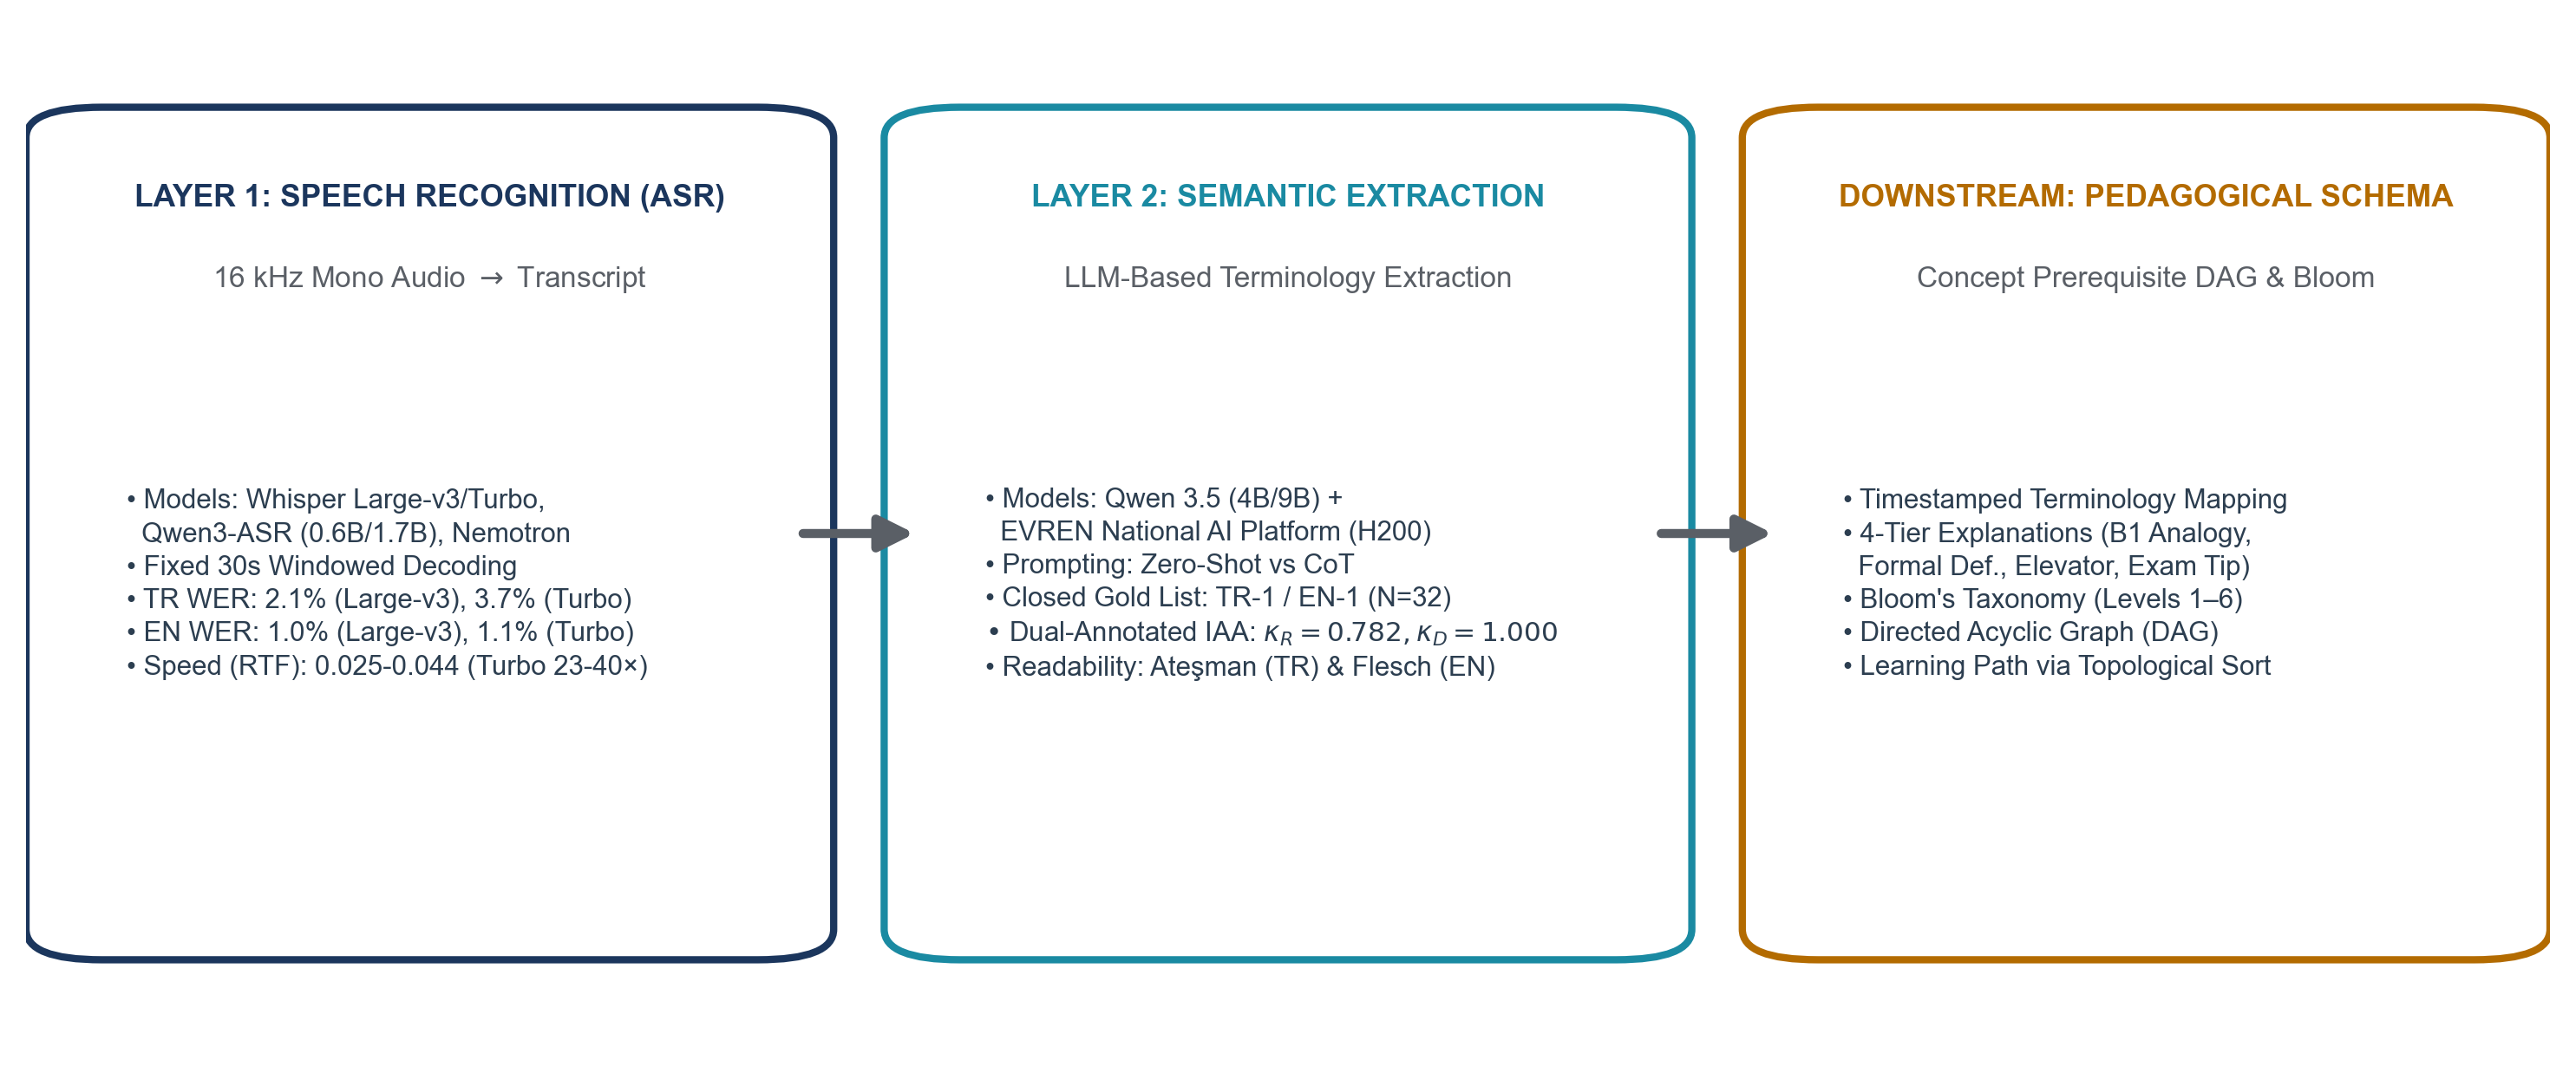
\includegraphics[width=\linewidth,height=8.3cm,keepaspectratio]{img/pipeline_architecture.png}
    \captionof{figure}{End-to-End Multilayer Architectural Pipeline.}

    \vskip0.4ex
    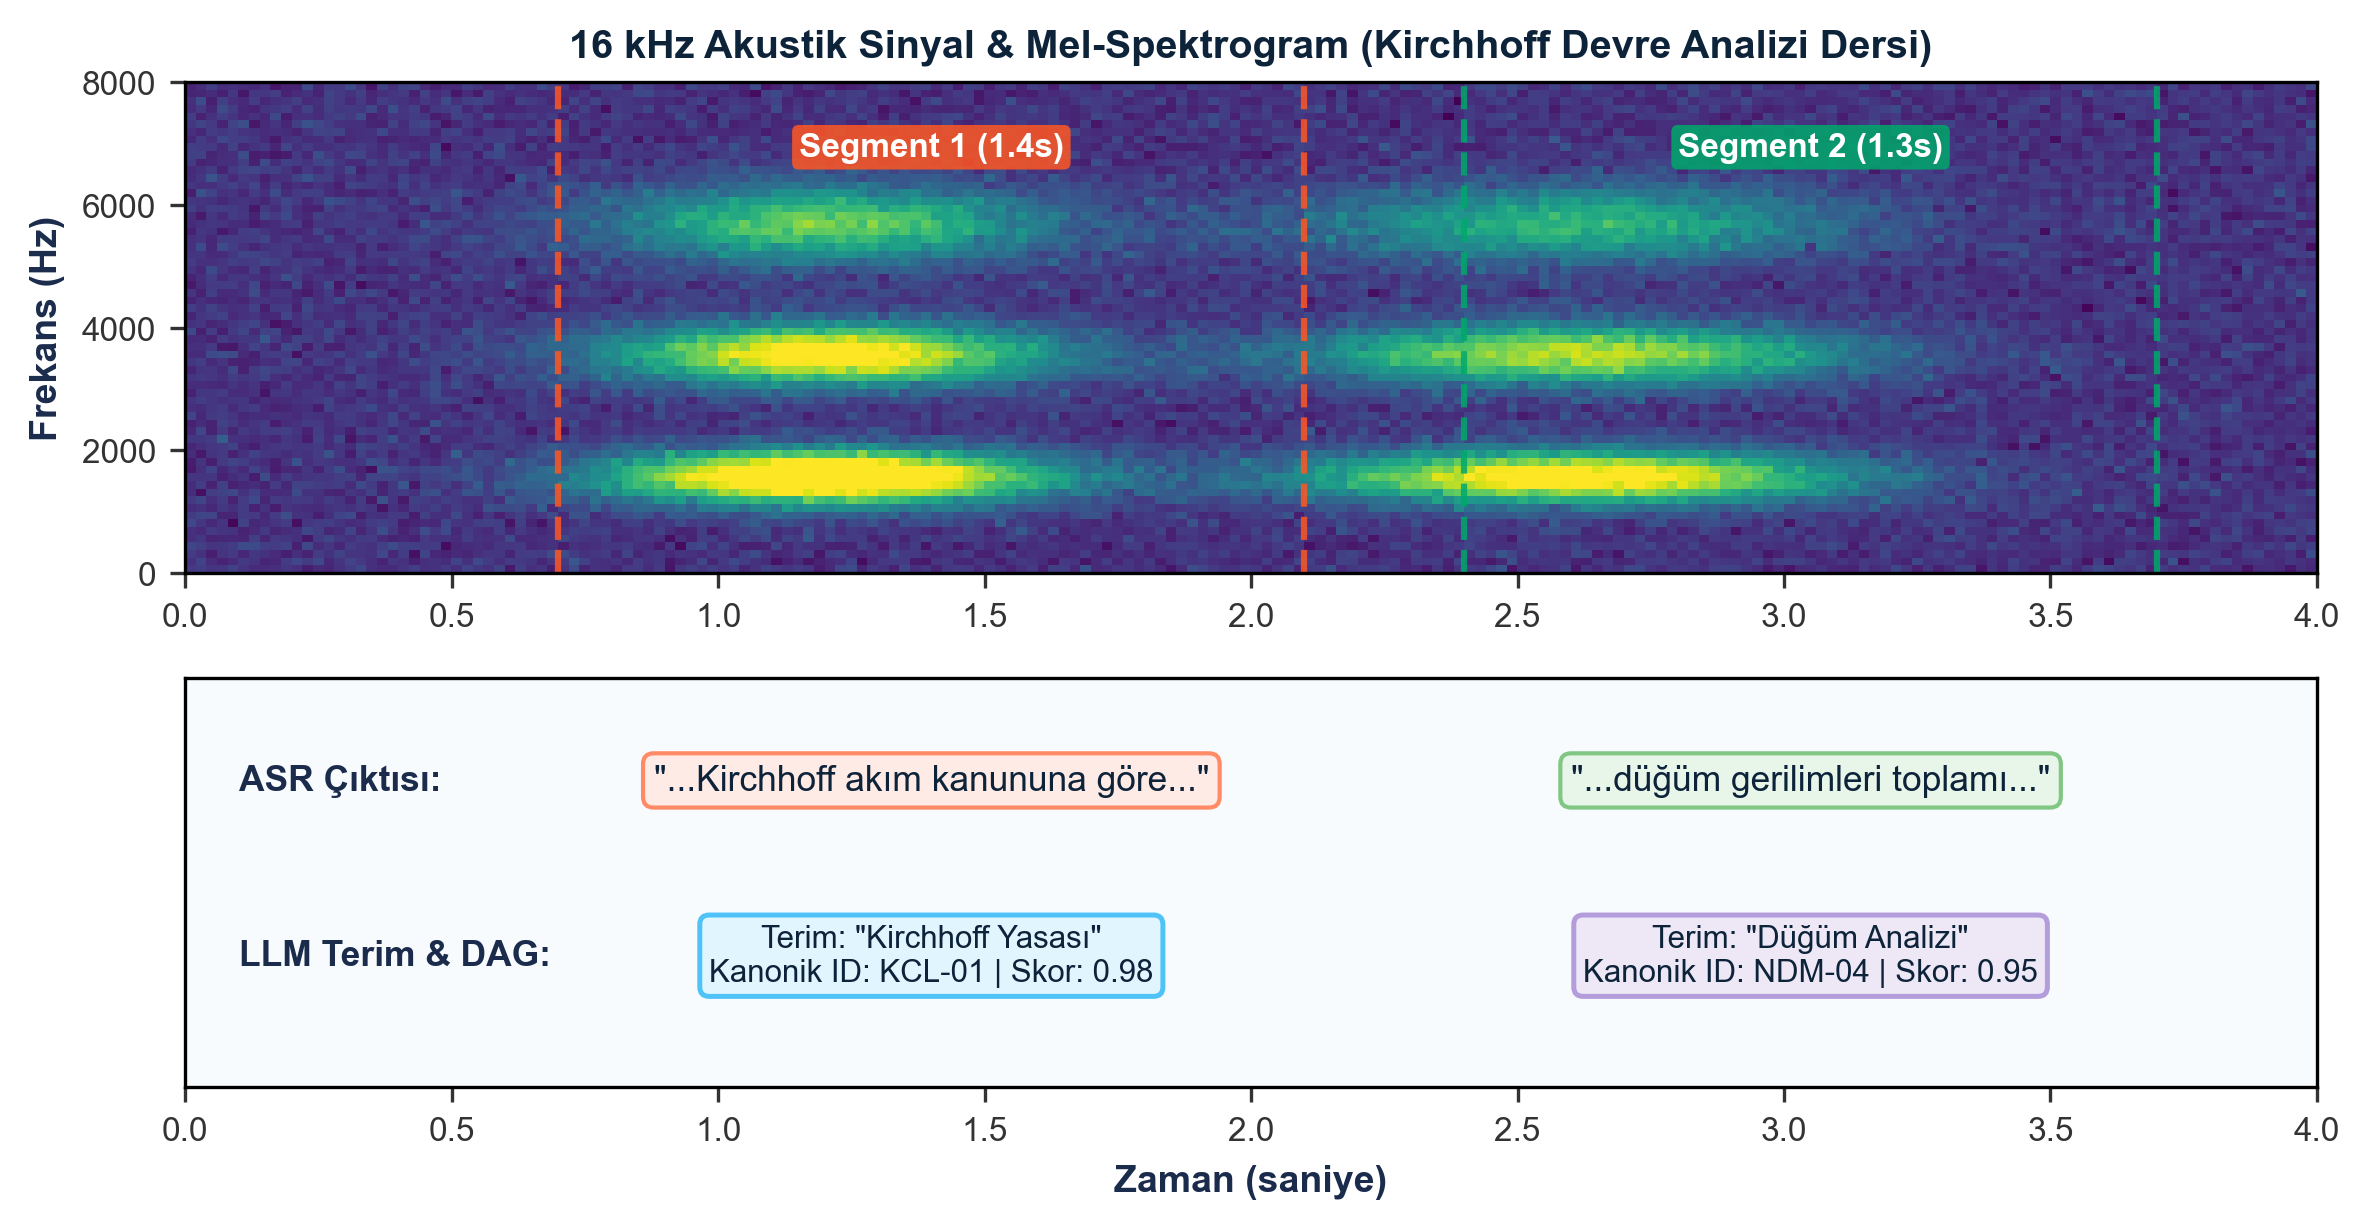
\includegraphics[width=\linewidth,height=7.9cm,keepaspectratio]{img/acoustic_spectrogram_extraction.png}
    \captionof{figure}{Acoustic Mel Spectrogram and Timestamped Term Extraction.}
  \end{block}

\end{column}

% =========================================================================
% COLUMN 2
% =========================================================================
\separatorcolumn

\begin{column}{\colwidth}

  \begin{block}{40-VIDEO EDUCATIONAL CORPUS}
    \begin{itemize}
      \item \textbf{12 Disciplines:} STEM, medicine, social sciences, and corporate compliance (KVKK/GDPR, OHS). 7-lecture verified core test set.
      \item \textbf{Inter-Annotator Agreement:} Double-annotation on $N=115$ items yields Cohen's $\kappa_R=0.782$ (context) and $\kappa_D=1.000$ (definition).
    \end{itemize}

    \vskip0.3ex
    \centering
    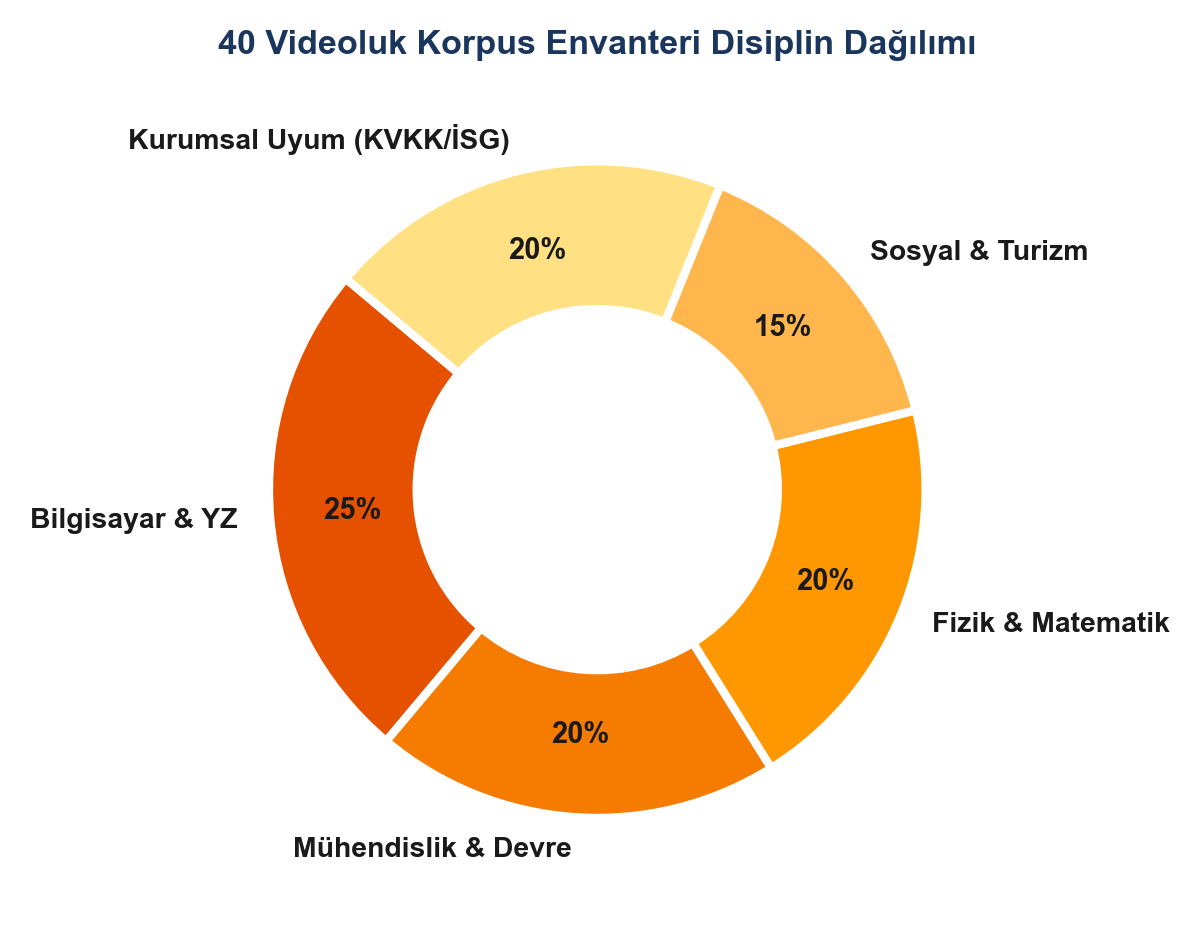
\includegraphics[width=0.92\linewidth,height=7.8cm,keepaspectratio]{img/chart_a_donut.png}
    \captionof{figure}{Corpus Discipline Distribution.}
  \end{block}

  \vskip-0.4ex
  \begin{block}{MULTILINGUAL ASR COMPARISON (WER)}
    \centering
    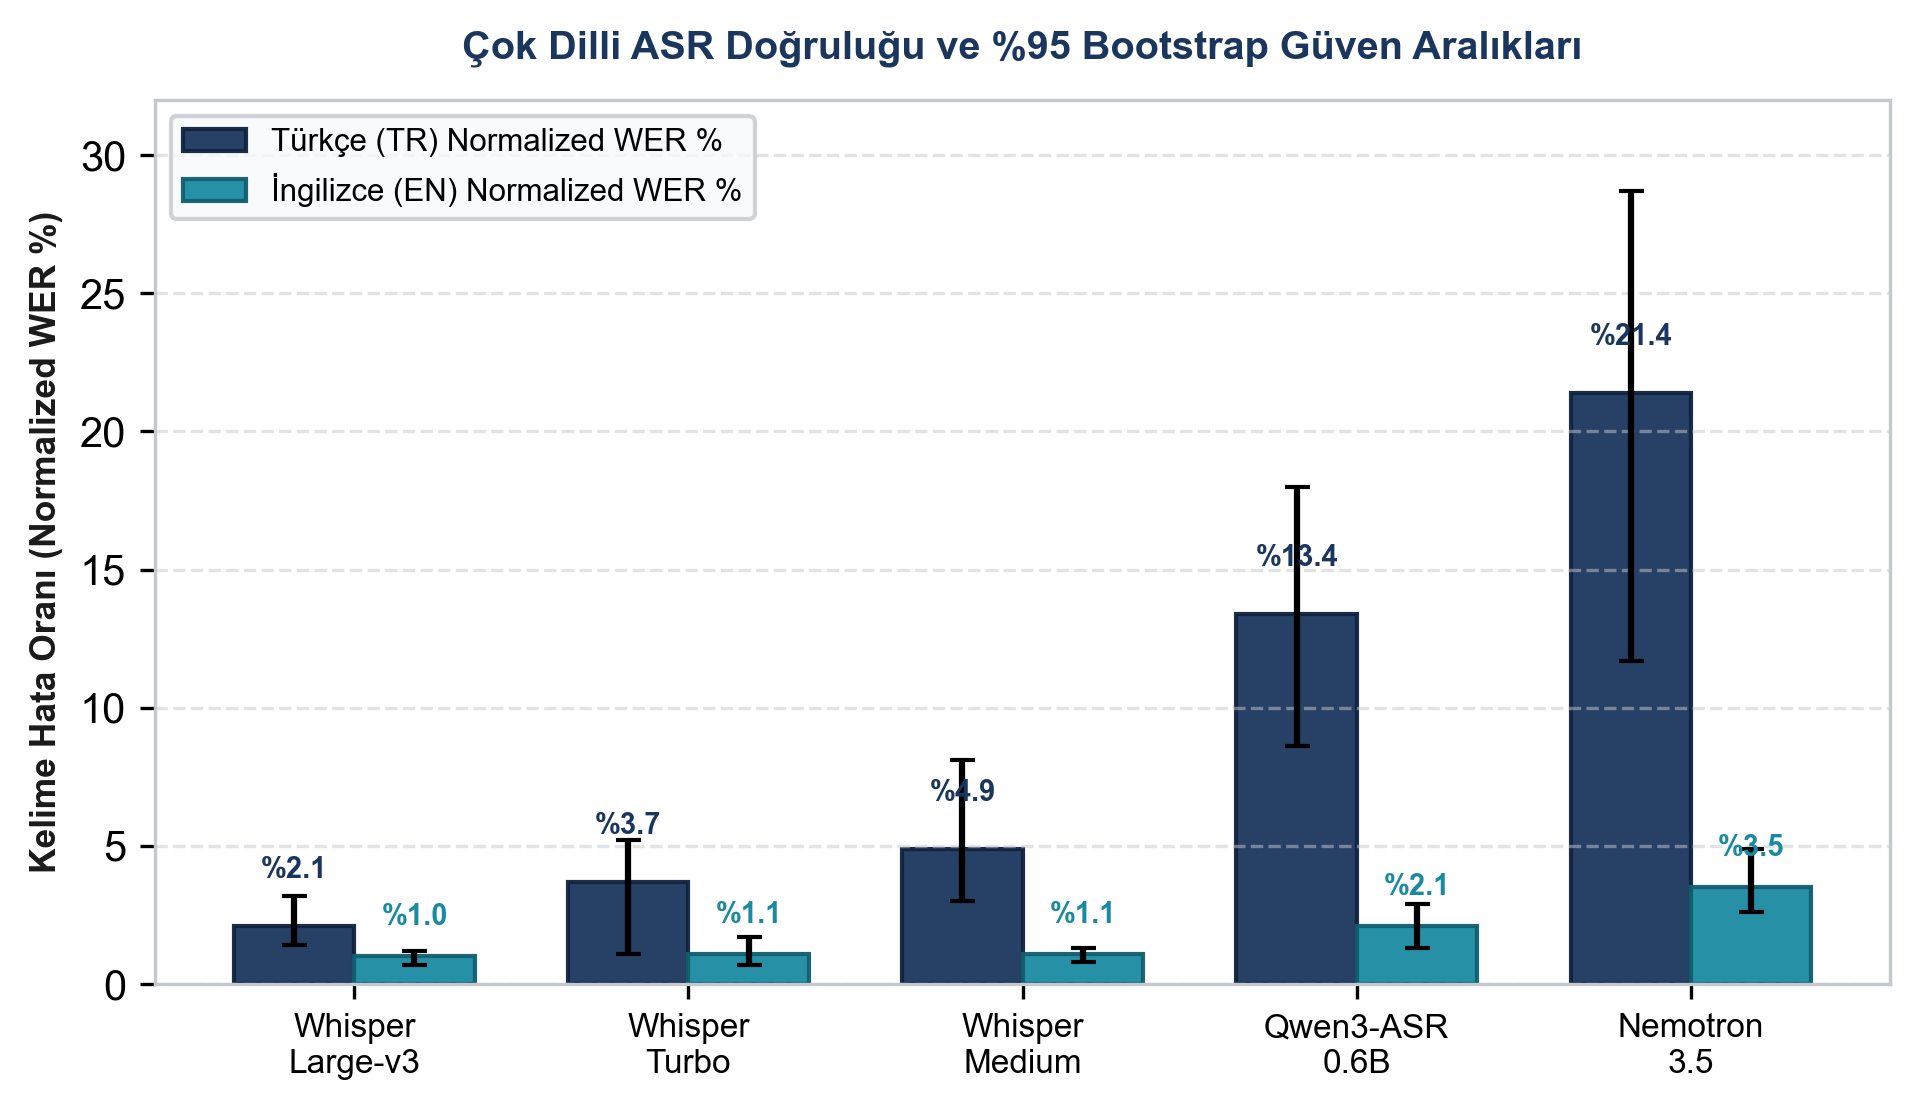
\includegraphics[width=\linewidth,height=7.8cm,keepaspectratio]{img/asr_benchmark_chart.png}
    \captionof{figure}{Normalized WER and 95\% Confidence Intervals ($B=10\,000$).}

    \begin{itemize}
      \item \textbf{Whisper Large-v3:} Peak accuracy with $2.1\%$ WER (TR) and $1.0\%$ (EN).
      \item \textbf{Whisper Turbo:} High-speed RTF $0.025$--$0.044$ ($23$--$40\times$ real-time).
      \item \textbf{VAD Degradation:} Energy-based VAD clips phonetic boundaries, degrading WER from $2.1\%$ to $4.1\%$.
    \end{itemize}
  \end{block}

  \vskip-0.4ex
  \begin{block}{TABLE 1: INFERENCE TIME COMPARISON}
    \small\setlength{\tabcolsep}{5pt}
    \renewcommand{\arraystretch}{1.25}
    \begin{tabularx}{\linewidth}{>{\raggedright\arraybackslash}X c c >{\raggedright\arraybackslash}X}
      \toprule
      \rowcolor{deepnavy}
      \textcolor{white}{\textbf{Model / Hardware}} & \textcolor{white}{\textbf{TR Time}} & \textcolor{white}{\textbf{EN Time}} & \textcolor{white}{\textbf{Platform}} \\
      \midrule
      \textbf{EVREN Qwen 3.8F} & \textbf{6.11 s} & \textbf{4.23 s} & National Cloud (H200) \\
      \textbf{Boğaziçi HPC (A40)} & \textbf{15.28 s} & \textbf{12.45 s} & 7B LoRA (48GB A40) \\
      \textbf{EVREN DeepSeek} & 27.68 s & 24.12 s & High Throughput \\
      \textbf{Qwen 3.5-4B (Local)} & 39.80 s & 34.20 s & RTX 5060 (4-bit NF4) \\
      \textbf{Qwen 3.5-9B (Local)} & 513.19 s & 322.29 s & CPU Offload \\
      \bottomrule
    \end{tabularx}
  \end{block}

\end{column}

% =========================================================================
% COLUMN 3
% =========================================================================
\separatorcolumn

\begin{column}{\colwidth}

  \begin{block}{BOĞAZİÇİ HPC A40 7B LoRA TRAINING}
    \begin{itemize}
      \item \textbf{Parameter-Efficient Adaptation:} \texttt{Qwen2.5-7B-Instruct} adapted with $r=16$, $\alpha=32$ on A40 (Job ID \texttt{33580}).
      \item \textbf{Resource Profile:} 3 epochs in \textbf{13.67 s}; peak VRAM \textbf{27.84 GB}.
      \item \textbf{Cross-Domain Gain:} CS/BST recall rose from $0.0\%$ to \textbf{33.3\%}; Ateşman readability improved by \textbf{+25.7 points} into B1.
    \end{itemize}

    \vskip0.3ex
    \centering
    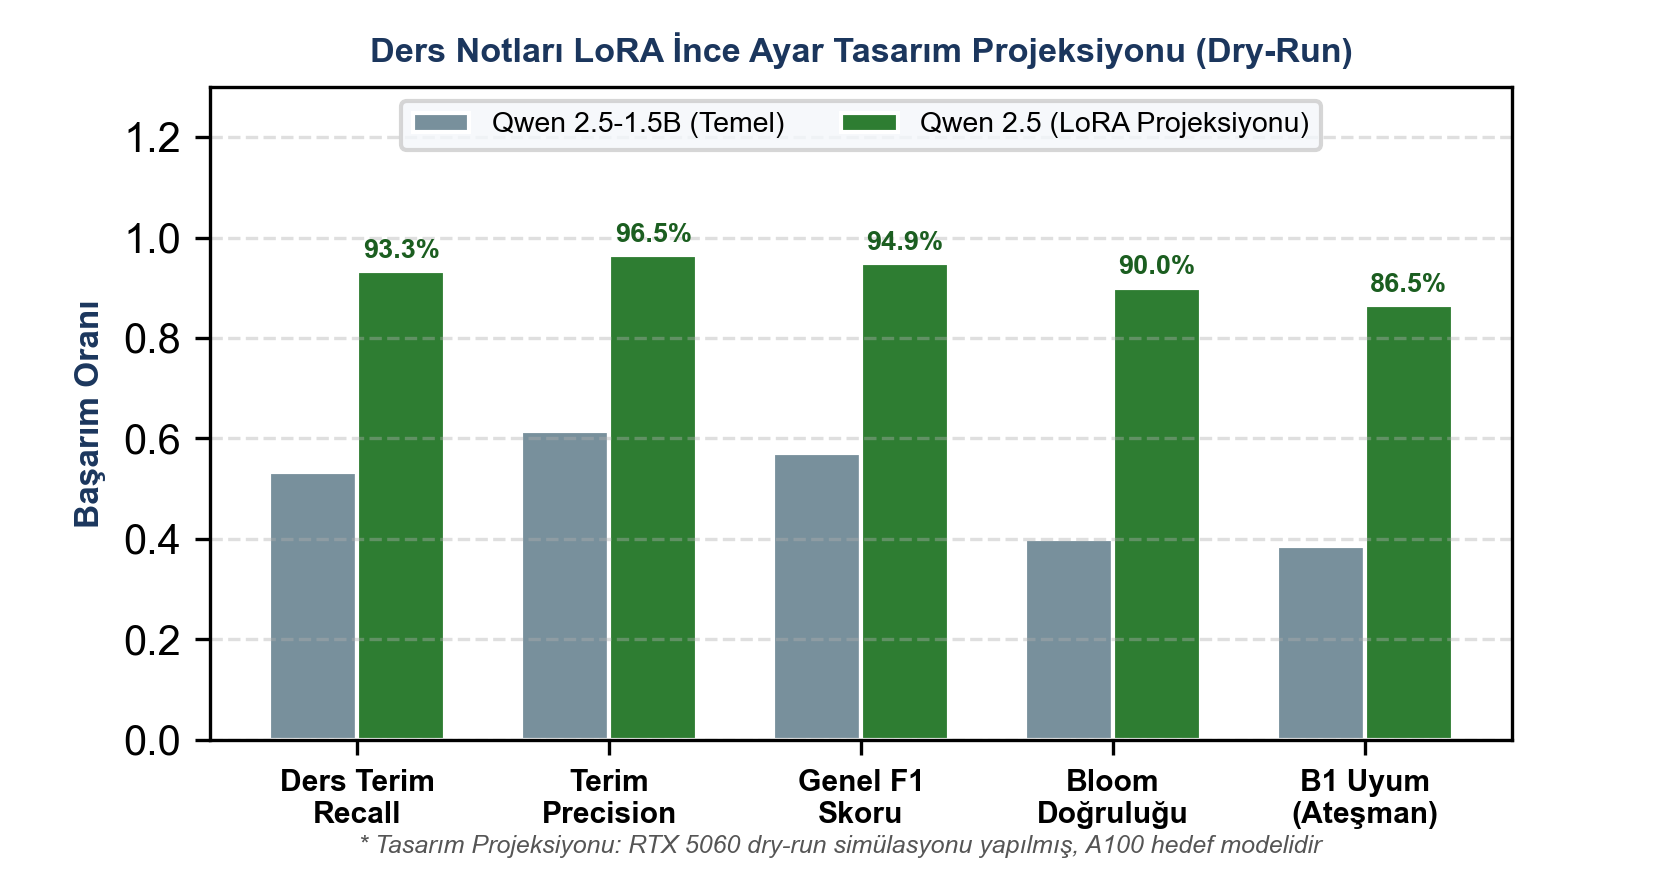
\includegraphics[width=\linewidth,height=7.0cm,keepaspectratio]{img/finetune_gain_chart.png}
    \captionof{figure}{Qwen 2.5-7B LoRA Adaptation and Readability Gain.}
  \end{block}

  \vskip-0.4ex
  \begin{block}{HYBRID RAG AND PREREQUISITE GRAPH}
    \centering
    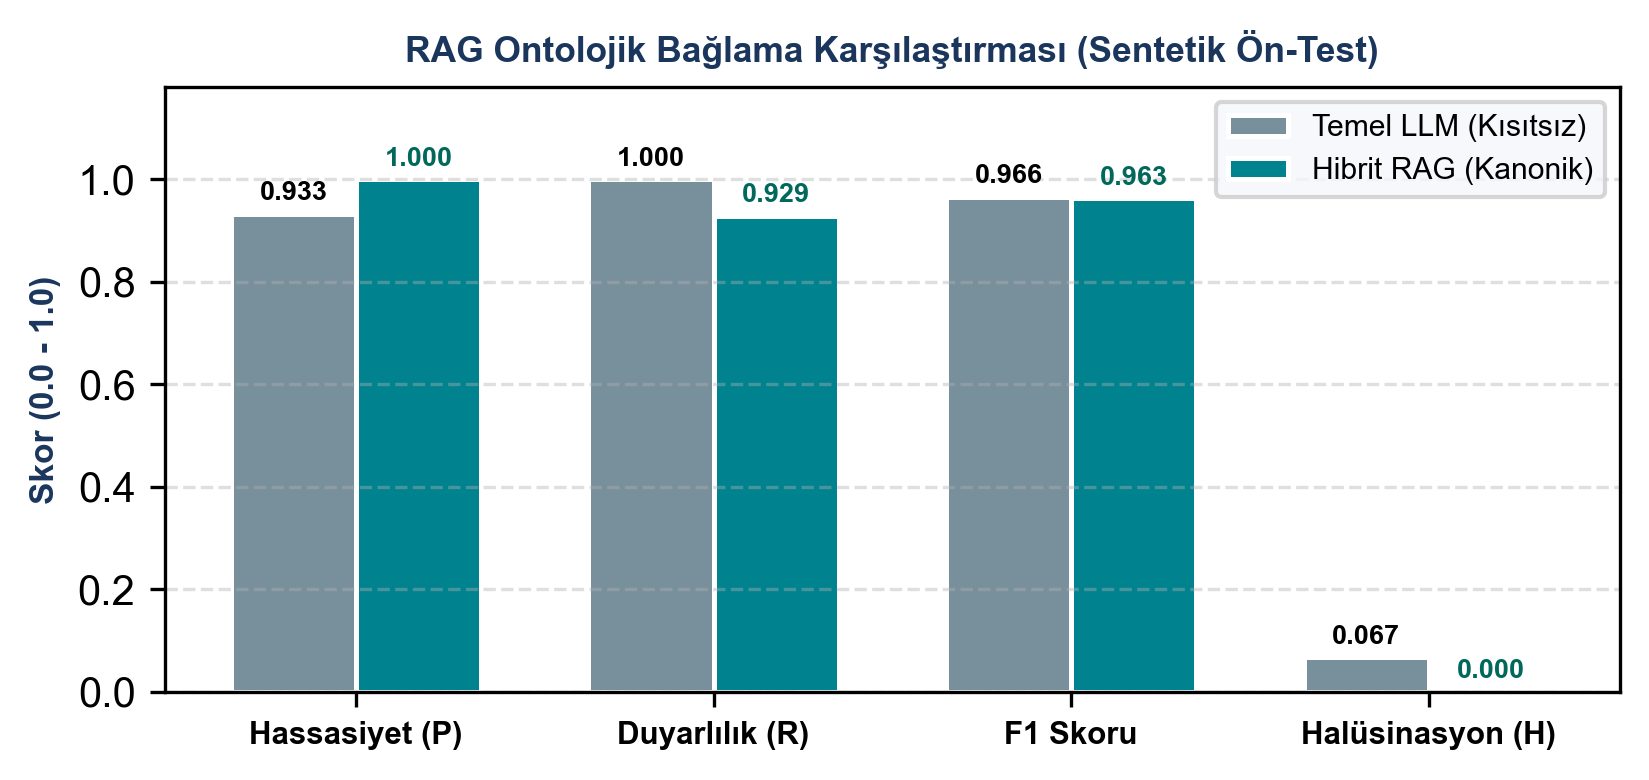
\includegraphics[width=\linewidth,height=6.7cm,keepaspectratio]{img/rag_performance_chart.png}
    \captionof{figure}{Hybrid RAG Grounding and Prerequisite Extraction.}

    \begin{itemize}
      \item \textbf{Knowledge Grounding:} Contextualizes technical concepts across 7 domain ontologies via BM25 + Dense RRF fusion.
      \item \textbf{Prerequisite Gap Detection:} Detects missing prerequisite concepts skipped during rapid lecture delivery.
    \end{itemize}
  \end{block}

  \vskip-0.4ex
  \begin{block}{CROSS-LAYER ERROR PROPAGATION}
    \centering
    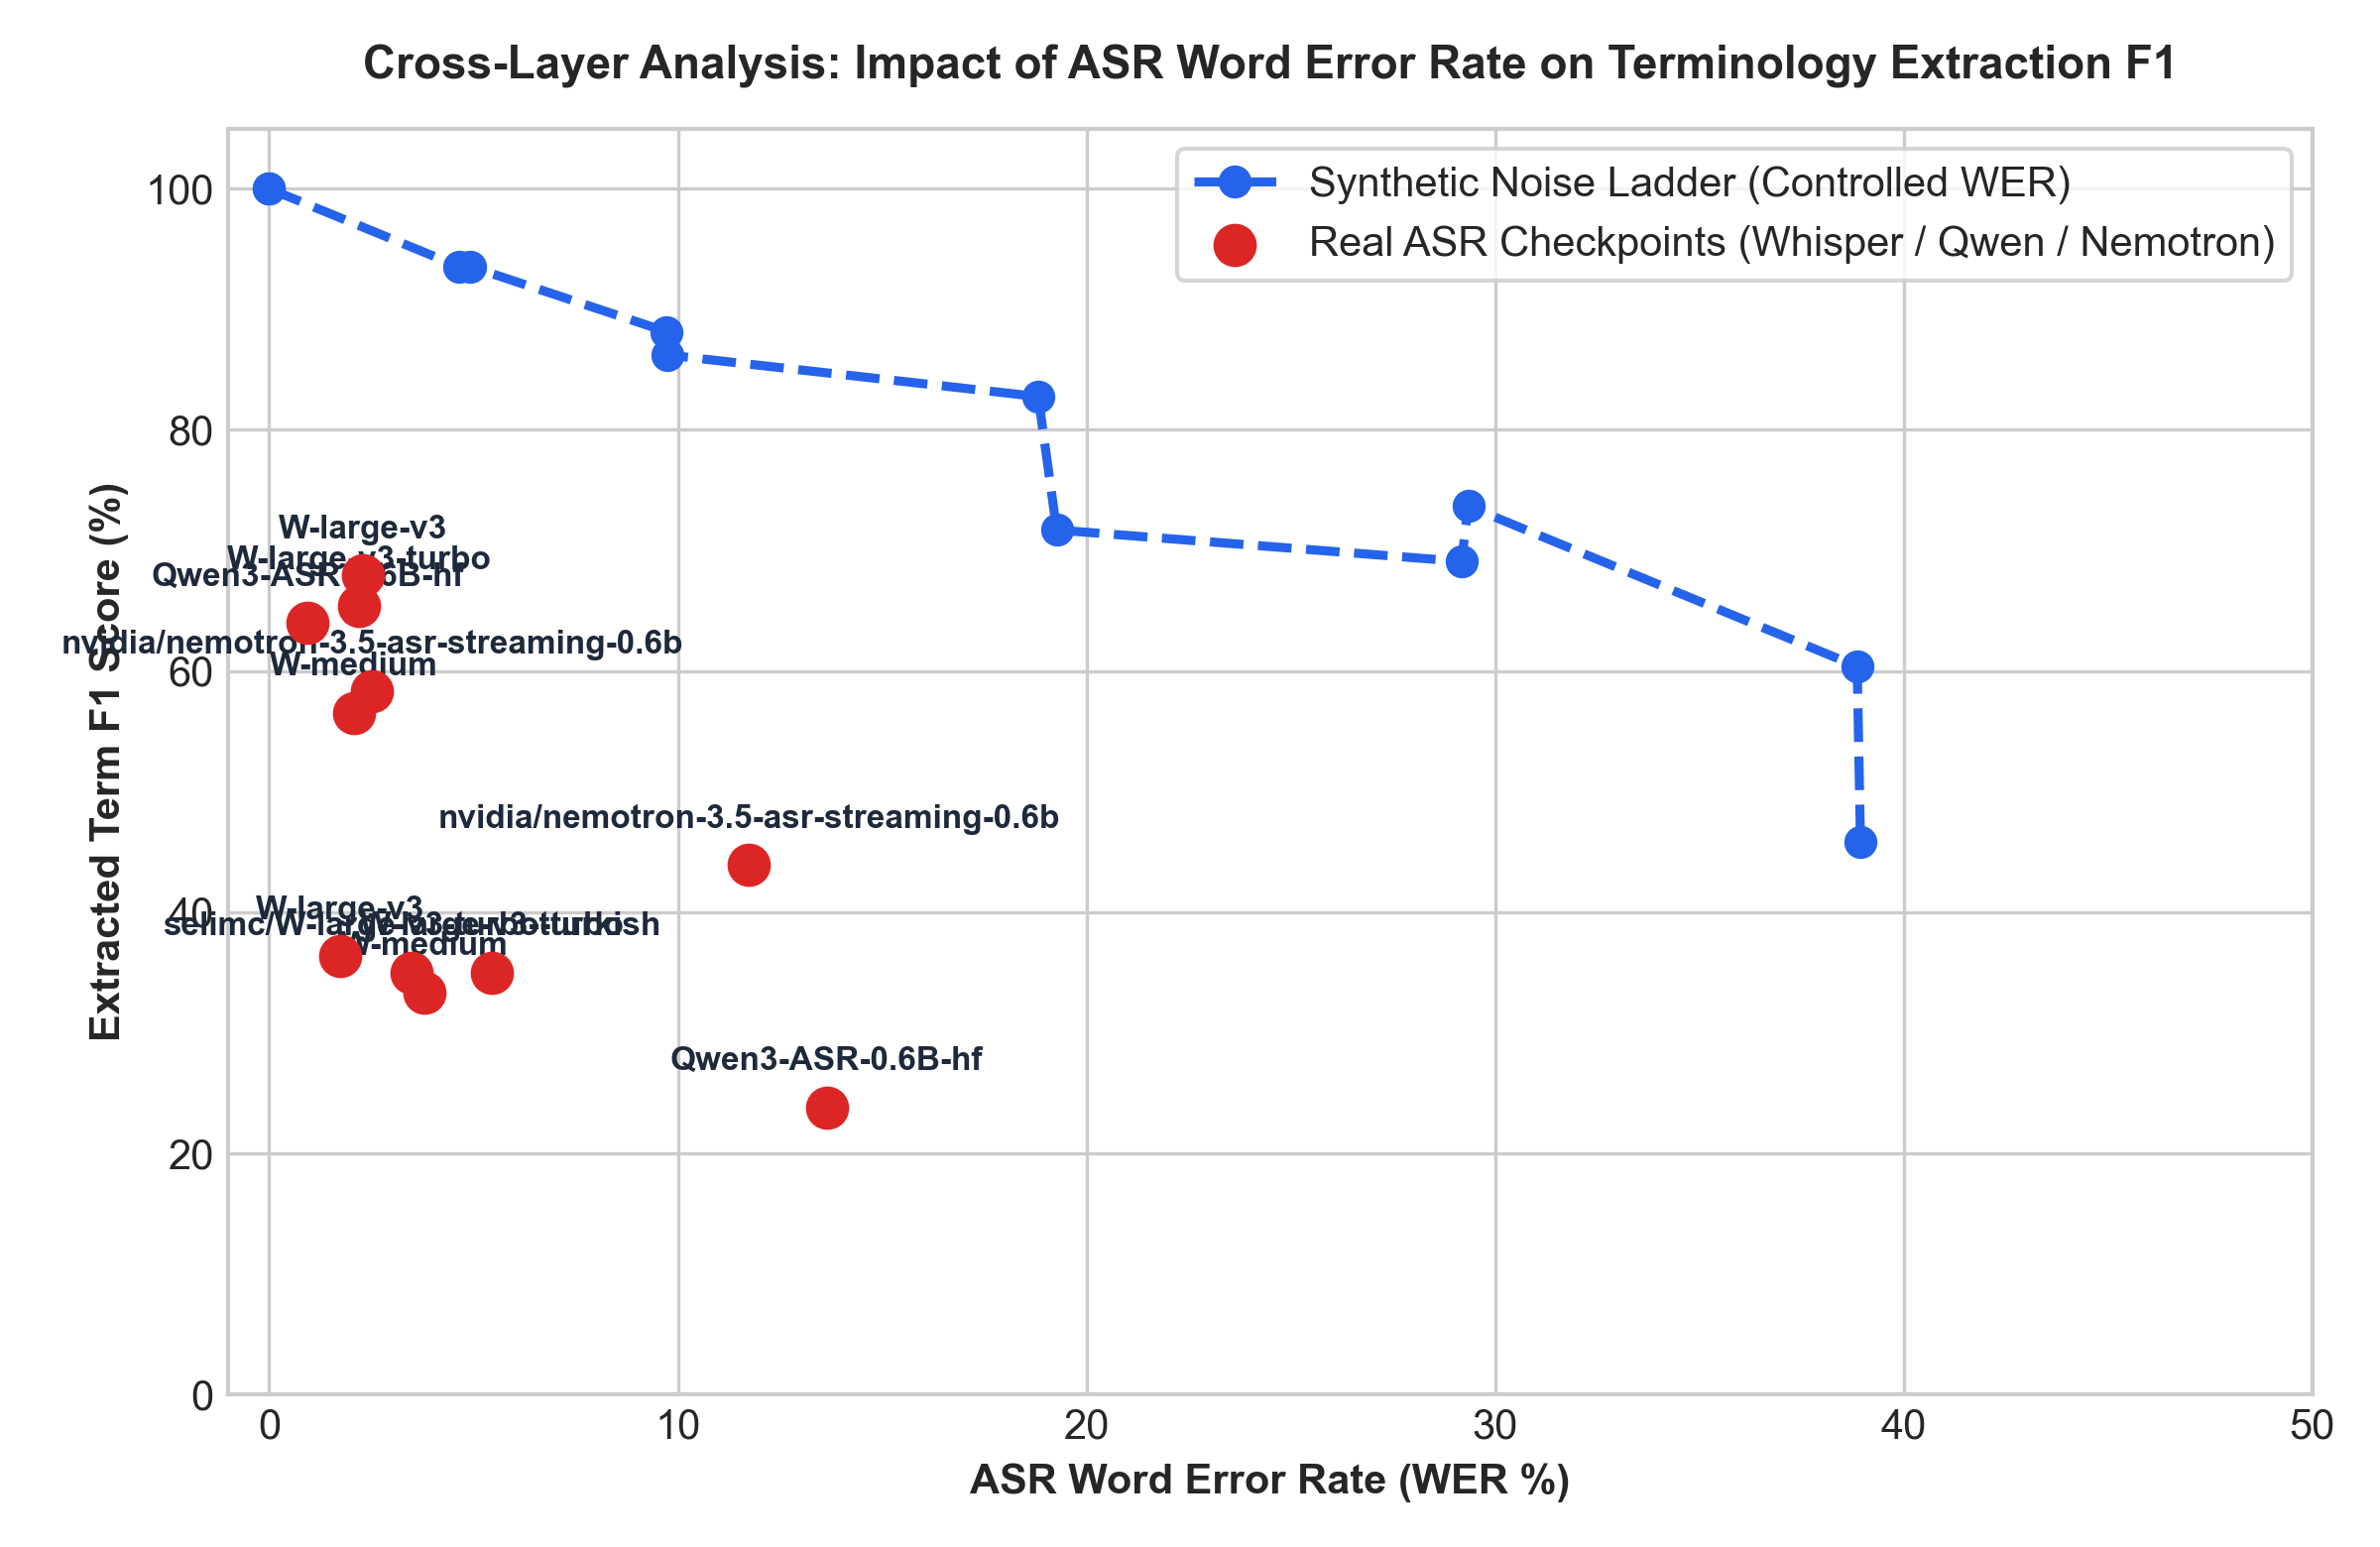
\includegraphics[width=\linewidth,height=6.5cm,keepaspectratio]{img/cross_layer_curve.png}
    \captionof{figure}{Empirical Error-Propagation Curves on HPC A40.}

    \begin{itemize}
      \item \textbf{Acoustic Ladder:} 7 ASR levels tested ($0\%$ to $89.7\%$ WER).
      \item \textbf{Sensitivity:} $\Delta\text{WER}=+5\% \implies \Delta F_1=-0.11\%$ (TR) / $-1.23\%$ (EN).
      \item \textbf{Tolerance:} At $\text{WER}\le15\%$, extraction stays stable; above $40\%$, hallucination surges to $91.7\%$.
    \end{itemize}
  \end{block}

\end{column}

% =========================================================================
% COLUMN 4
% =========================================================================
\separatorcolumn

\begin{column}{\colwidth}

  \begin{block}{FULL-CORPUS DAG AND PREREQUISITE GAPS}
    \begin{itemize}
      \item \textbf{33 Lectures Analyzed:} Full corpus processed on A40 in 504.47~s ($\sim$8.4~min), extracting \textbf{118 technical terms} and topological dependency paths.
      \item \textbf{Pedagogical Gaps Identified:} 19 gaps detected (7 in KVKK, 5 each in OHS), highlighting concepts introduced without prerequisites.
      \item \textbf{CEFR-B1 Clarity:} \textbf{57.6\%} of generated explanations fall in B1 band.
    \end{itemize}

    \vskip0.3ex
    \centering
    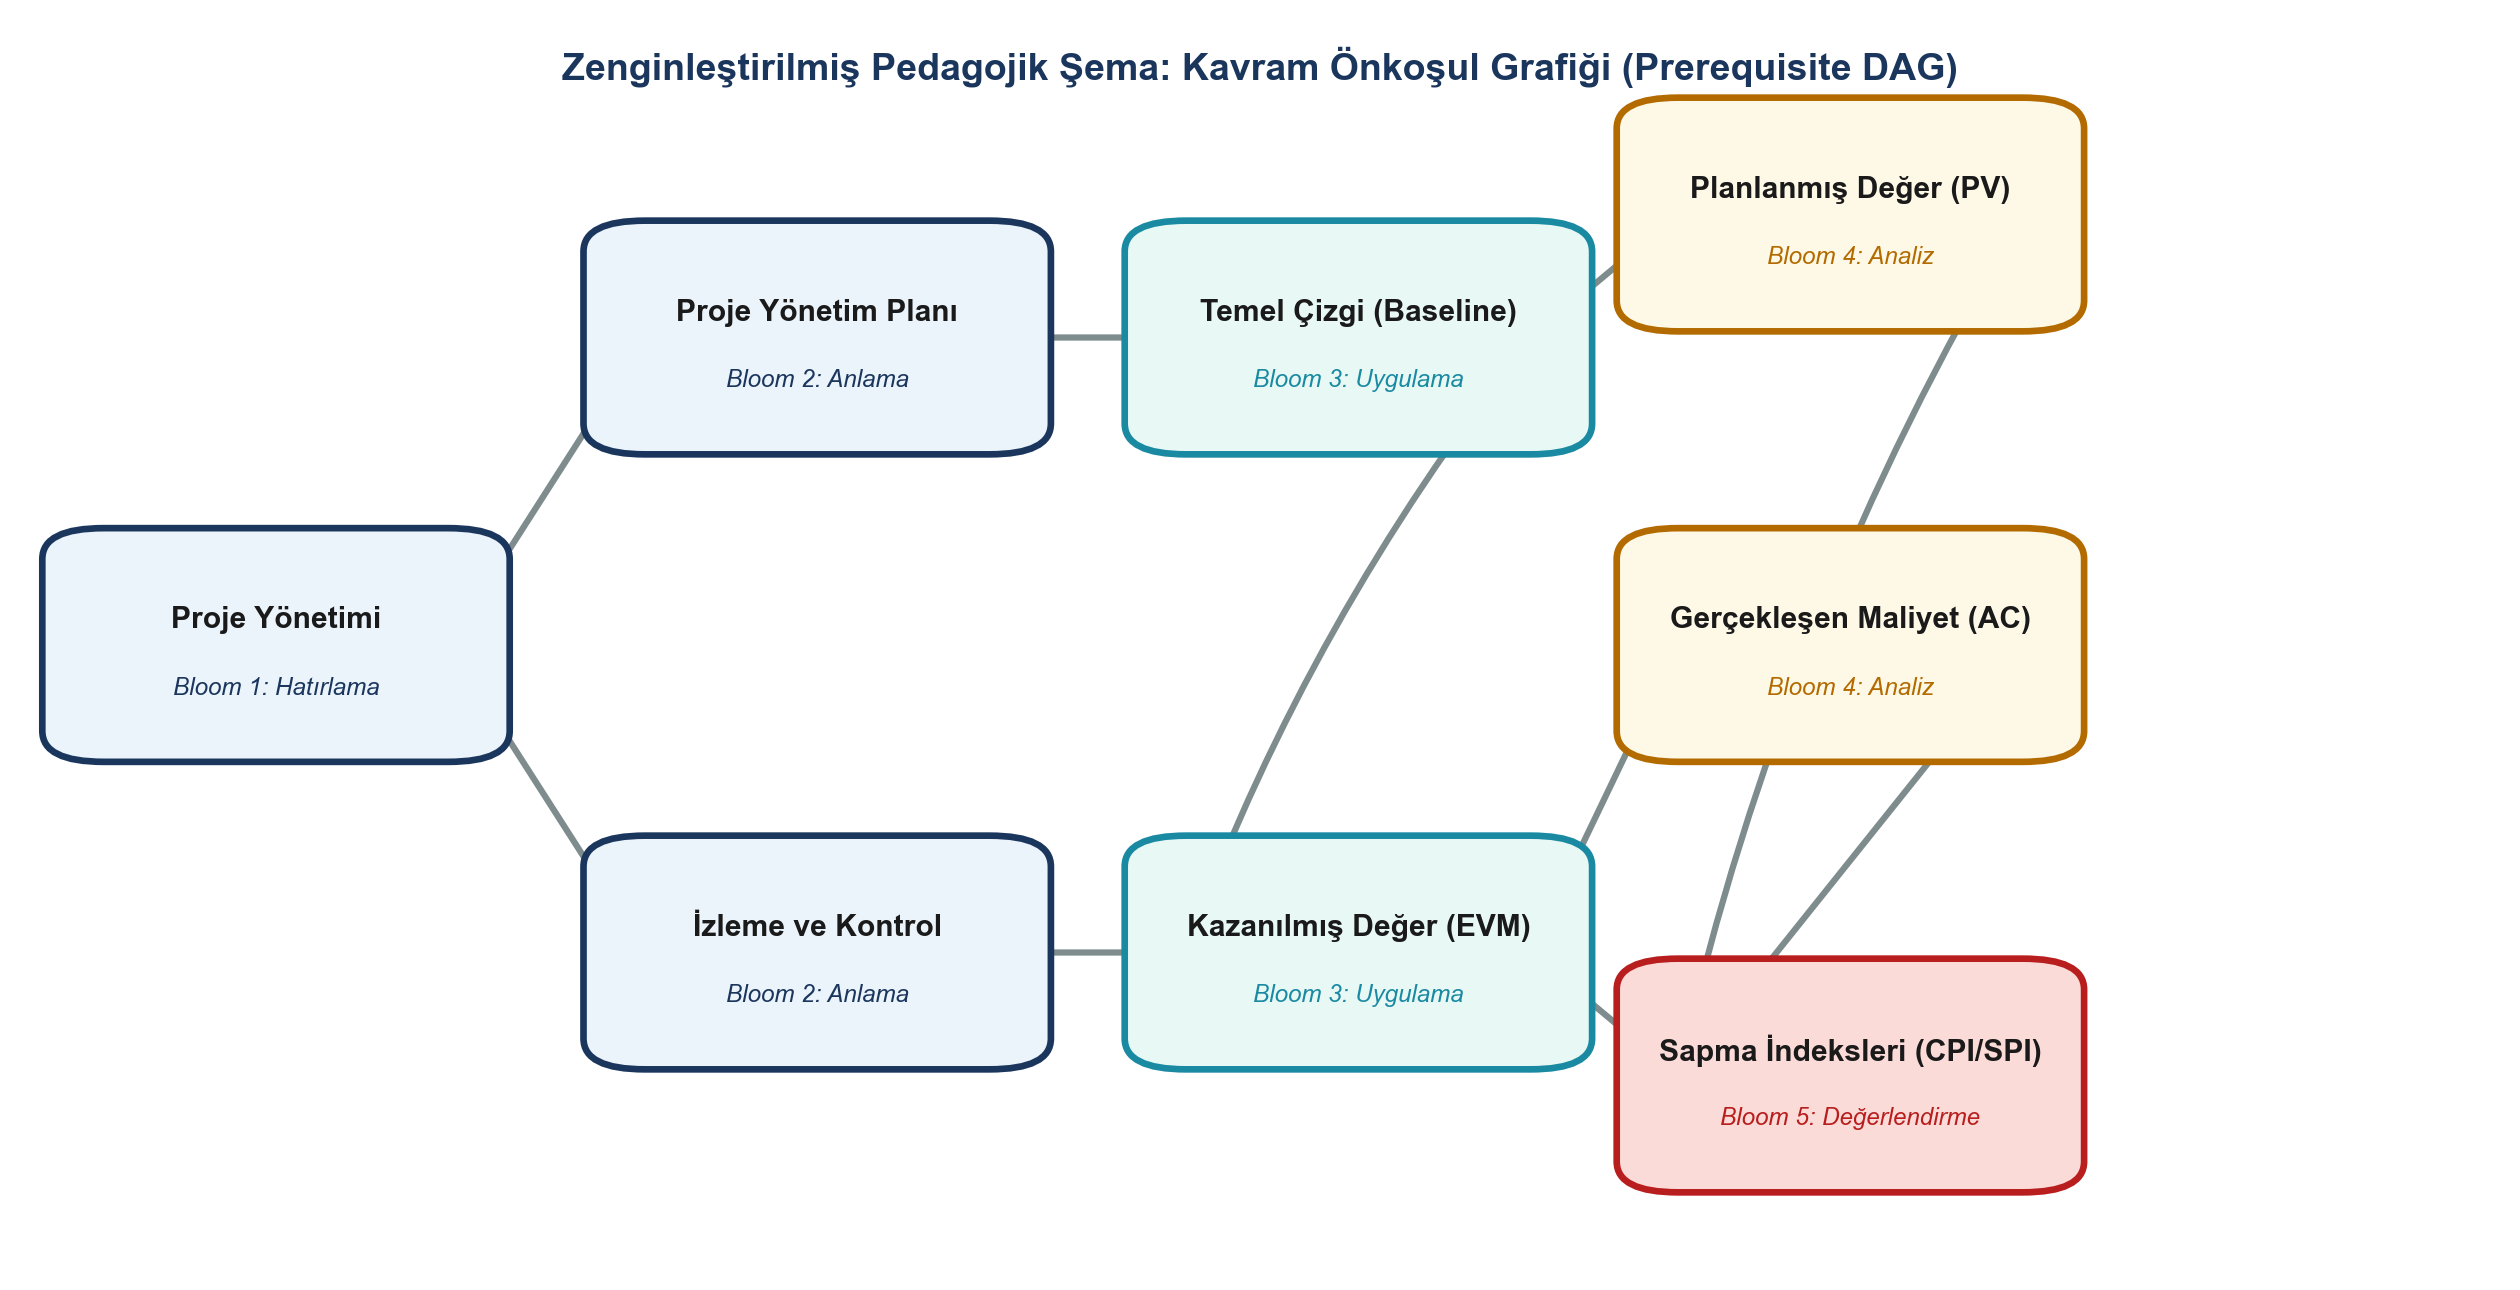
\includegraphics[width=\linewidth,height=7.4cm,keepaspectratio]{img/concept_dag_graph.png}
    \captionof{figure}{Concept Dependency Graph and Bloom Hierarchy.}
  \end{block}

  \vskip-0.4ex
  \begin{block}{TABLE 2: COMPETITIVE PLATFORM MATRIX}
    \small\setlength{\tabcolsep}{5pt}
    \renewcommand{\arraystretch}{1.25}
    \begin{tabularx}{\linewidth}{>{\raggedright\arraybackslash}X c c c}
      \toprule
      \rowcolor{deepnavy}
      \textcolor{white}{\textbf{Feature}} & \textcolor{white}{\textbf{EduTerm AI}} & \textcolor{white}{\textbf{Coursera / edX}} & \textcolor{white}{\textbf{Duolingo}} \\
      \midrule
      \textbf{ASR Term Extraction} & \textbf{Automated} & Manual Subtitles & Limited \\
      \textbf{Canonical RAG} & \textbf{Yes (Hybrid)} & No & No \\
      \textbf{Prerequisite DAG} & \textbf{Yes (NetworkX)} & Static Course Tree & Linear Tree \\
      \textbf{Edge / Private Inference} & \textbf{Yes (Local/Web)} & Cloud Only & Cloud API \\
      \textbf{CEFR-B1 Scaffolding} & \textbf{Yes (Ateşman)} & None & Fixed A1--B2 \\
      \bottomrule
    \end{tabularx}
  \end{block}

  \vskip-0.4ex
  \begin{block}{RESULTS AND CONCLUSION}
    \begin{itemize}
      \item \textbf{Practical Viability:} Verified end-to-end multi-tier pipeline on Boğaziçi HPC (A40) and local RTX 5060; SLMs enable private edge tutoring.
      \item \textbf{Future Work:} Real-time LMS integration (Canvas/Moodle) and continuous student BKT knowledge tracing.
    \end{itemize}
  \end{block}

  \vskip-0.4ex
  \begin{block}{ACKNOWLEDGMENTS}
    \footnotesize
    Conducted under Boğaziçi University CMPE 492. Computational infrastructure supported by Boğaziçi University Computer Engineering HPC Cluster (NVIDIA A40 48GB), SSB / TÜBİTAK BİLGEM National EVREN AI Platform (NVIDIA H200), and Tatilsepeti R\&D Center.
  \end{block}

\end{column}

\separatorcolumn
\end{columns}
\end{frame}

\end{document}
